\section{Introduction}
Human land use has had a big impact on the structure of landscapes~\citep{turner1989landscape}. Many landscapes have been divided into patches by human created linear landscape elements (e.g. roads, waterways, tree lines and hedges) \citep{meyer2012multifunctional}. This creates a mosaic with a combination of natural and human influenced landscapes of varying sizes and shapes. These patches and their connectivity influence the ecology of the landscape: it effects the distribution of species and the dispersal of seeds, the flow of matter and nutrients, and the water balance~\citep{turner1989landscape}.

Linear elements, such as roads and railways, form barriers which lead to habitat fragmentation, while others, such as hedgerows and tree lines, can form corridors for animals and plants between patches~\citep{spellerberg1999introduction}. They also control fluxes, like the flow of water and pollutants via ditches, and by influencing air flow by, for example, tree lines and hedges~\citep{burel1996hedgerows}. Furthermore they provide habitats for species who are otherwise not able to live in the agricultural landscape~\citep{spellerberg1999introduction}.

Agriculture has been an important factor in the creation of linear elements, leading to a mosaic landscape. Linear features like ditches, lynchets and hedgerows are often the result of agricultural practices~\citep{bailly2008agrarian}. They have therefore become an important part of the European landscape, which is dominated by agriculture. Intensification of arable farming in Europe has led to larger agricultural fields, simpler crop rotations and a reduction in non-crop features. Consequently the diversity in the landscape and occurrence of linear elements has diminished~\citep{stoate2001ecological}. Thus increasing the importance of the remaining linear features.

Not only do these linear elements have an ecological significance, some also have a cultural value~\citep{jongman2004landscape}. Linear elements, like tree lines, hedges, waterways and ditches, are often considered traditional and aesthetically pleasing, and are therefore part of natural heritage~\citep{gobster2007shared}.

\medskip

Given the significance of linear landscape elements within the European landscape an assessment of the coverage of these elements would be beneficial~\citep{van2013modelling,bailly2008agrarian}. There are multiple ways to approach this. \citet{van2013modelling}, for example, used over 200,000 ground observations within the European Union of linear landscape elements and used interpolation to create a map of the density of linear landscape elements in the European Union. This approach can certainly be useful to estimate linear elements in the landscape, but interpolation introduces an unknown error. A more precise way of assessing the presence of linear elements in the landscape could be identification using remote sensing. This could be done by using high resolution aerial imagery, by using airborne LiDAR (Light Detecting and Ranging), which uses lasers to determine height by measuring the time it takes for the laser to be reflected back~\citep{lefsky2002lidar,lim2003lidar}, or by combining these two.

Scanning the earth using lasers leads to Very High Resolution (VHR) elevation data, often with multiple observation points per square meter and thus provides a very detailed 3D image of the landscape~\citep{lefsky2002lidar}. Airborne LiDAR datasets with high point density are becoming increasingly available. Countries like the Netherlands and Denmark, for example, have made LiDAR datasets of the entire country freely accessible~\citep{AHN2016inwinjaren, SDFE2017dhm}.

Airborne LiDAR often has two additional properties which are very useful for detecting vegetation:
\begin{enumerate*}[(i)]
	\item multiple returns, and
	\item intensity of the backscattered signal.
\end{enumerate*}
When a signal only partly reflects on an object, multiple return values can be recorded (figure~\ref{fig:LiDAR}).
Vegetation partly reflects the signal leading to multiple return values, including a last ground return. The shape of vegetation can be extracted using the different return values at a point~\citep{lim2003lidar}. The intensity describes the strength of the returning light (figure~\ref{fig:LiDAR}).
This is dependent on the surface on which it reflected and therefore provides meaningful information on the surface origin~\citep{song2002assessing}.
\begin{figure}
	\centering
	\fbox{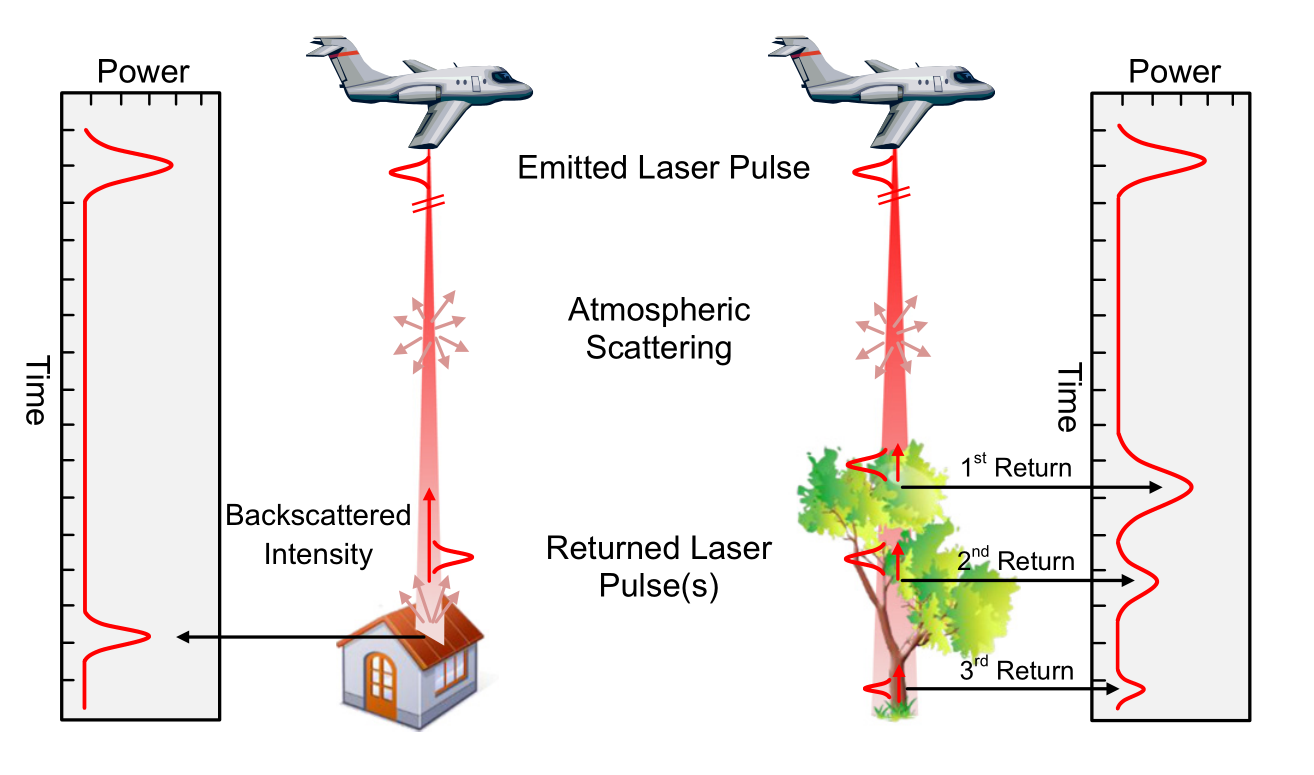
\includegraphics[scale=0.45]{./img/LiDAR}}
	\caption{The retrieval of airborne LiDAR data, resulting in backscatters of varying intensities and discrete returns~\citep{yan2015urban}.}
	\label{fig:LiDAR}
\end{figure}

\medskip

There are generally two main strategies to classify point clouds:
\begin{enumerate*}[(i)]
	\item create derived raster images (e.g. a DSM and DTM) and use conventional raster based techniques for classification, or
	\item classify the raw point cloud directly using machine learning algorithms~\citep{yan2015urban}.
\end{enumerate*}
Using derived raster images for classification is fairly straightforward and can lead to desirable results~\citep{maas1999potential, charaniya2004supervised, brennan2006object, forlani2006complete, antonarakis2008object, im2008object}, but a lot of detail is lost in the conversion from points to raster cells. Therefore directly classifying the point cloud is a more preferred method. Different machine learning algorithms are being tested and used for LiDAR datasets, for example Support Vector Machines (SVM)~\citep{mallet2008analysis, zhang2013svm, weinmann2015semantic}, Random Forest (RF)~\citep{chehata2009airborne, guo2011relevance, niemeyer2014contextual, weinmann2014semantic, weinmann2015semantic}, Markov Random Fields (MRF), Conditional Random Fields (CRF)~\citep{niemeyer2011conditional, niemeyer2012conditional, niemeyer2014contextual}, and Adaboost~\citep{lodha2007aerial, weinmann2015semantic}.

\medskip

After classification of the point cloud the linear objects need to be identified. The identification of linear features has been extensively researched for raster-based imagery. Mainly focussing on the automated delineation of roads from remotely sensed imagery. This process is often done in three steps:
\begin{enumerate*}[(i)]
	\item edge detection,
	\item road tracking, and
	\item road linking~\citep{quackenbush2004review}.
\end{enumerate*}
These methods generally work well for roads partly due to the structured nature of a road system. Vegetation is a lot more complex, having lines and patches in all kinds of shapes and sizes. This makes these raster-based techniques difficult to apply to an extraction of linear vegetation elements from points clouds.

In this paper we describe our method to delineate linear objects within vegetation using LiDAR point clouds. To achieve this we use a machine learning algorithm to classify vegetation points based on properties of the LiDAR points and computed neighbourhood parameters. To delineate linear objects within the vegetation points we present a novel way of using a region growing technique to segment the point cloud into rectangular objects. These objects are subsequently checked for linearity based on their elongatedness. The method is validated by comparing the results with manually acquired reference data.
